% Options for packages loaded elsewhere
\PassOptionsToPackage{unicode}{hyperref}
\PassOptionsToPackage{hyphens}{url}
%
\documentclass[
]{article}
\usepackage{lmodern}
\usepackage{amssymb,amsmath}
\usepackage{ifxetex,ifluatex}
\ifnum 0\ifxetex 1\fi\ifluatex 1\fi=0 % if pdftex
  \usepackage[T1]{fontenc}
  \usepackage[utf8]{inputenc}
  \usepackage{textcomp} % provide euro and other symbols
\else % if luatex or xetex
  \usepackage{unicode-math}
  \defaultfontfeatures{Scale=MatchLowercase}
  \defaultfontfeatures[\rmfamily]{Ligatures=TeX,Scale=1}
\fi
% Use upquote if available, for straight quotes in verbatim environments
\IfFileExists{upquote.sty}{\usepackage{upquote}}{}
\IfFileExists{microtype.sty}{% use microtype if available
  \usepackage[]{microtype}
  \UseMicrotypeSet[protrusion]{basicmath} % disable protrusion for tt fonts
}{}
\makeatletter
\@ifundefined{KOMAClassName}{% if non-KOMA class
  \IfFileExists{parskip.sty}{%
    \usepackage{parskip}
  }{% else
    \setlength{\parindent}{0pt}
    \setlength{\parskip}{6pt plus 2pt minus 1pt}}
}{% if KOMA class
  \KOMAoptions{parskip=half}}
\makeatother
\usepackage{xcolor}
\IfFileExists{xurl.sty}{\usepackage{xurl}}{} % add URL line breaks if available
\IfFileExists{bookmark.sty}{\usepackage{bookmark}}{\usepackage{hyperref}}
\hypersetup{
  pdftitle={Workflow for AFRP CPUE Data},
  pdfauthor={Montana},
  hidelinks,
  pdfcreator={LaTeX via pandoc}}
\urlstyle{same} % disable monospaced font for URLs
\usepackage[margin=1in]{geometry}
\usepackage{color}
\usepackage{fancyvrb}
\newcommand{\VerbBar}{|}
\newcommand{\VERB}{\Verb[commandchars=\\\{\}]}
\DefineVerbatimEnvironment{Highlighting}{Verbatim}{commandchars=\\\{\}}
% Add ',fontsize=\small' for more characters per line
\usepackage{framed}
\definecolor{shadecolor}{RGB}{248,248,248}
\newenvironment{Shaded}{\begin{snugshade}}{\end{snugshade}}
\newcommand{\AlertTok}[1]{\textcolor[rgb]{0.94,0.16,0.16}{#1}}
\newcommand{\AnnotationTok}[1]{\textcolor[rgb]{0.56,0.35,0.01}{\textbf{\textit{#1}}}}
\newcommand{\AttributeTok}[1]{\textcolor[rgb]{0.77,0.63,0.00}{#1}}
\newcommand{\BaseNTok}[1]{\textcolor[rgb]{0.00,0.00,0.81}{#1}}
\newcommand{\BuiltInTok}[1]{#1}
\newcommand{\CharTok}[1]{\textcolor[rgb]{0.31,0.60,0.02}{#1}}
\newcommand{\CommentTok}[1]{\textcolor[rgb]{0.56,0.35,0.01}{\textit{#1}}}
\newcommand{\CommentVarTok}[1]{\textcolor[rgb]{0.56,0.35,0.01}{\textbf{\textit{#1}}}}
\newcommand{\ConstantTok}[1]{\textcolor[rgb]{0.00,0.00,0.00}{#1}}
\newcommand{\ControlFlowTok}[1]{\textcolor[rgb]{0.13,0.29,0.53}{\textbf{#1}}}
\newcommand{\DataTypeTok}[1]{\textcolor[rgb]{0.13,0.29,0.53}{#1}}
\newcommand{\DecValTok}[1]{\textcolor[rgb]{0.00,0.00,0.81}{#1}}
\newcommand{\DocumentationTok}[1]{\textcolor[rgb]{0.56,0.35,0.01}{\textbf{\textit{#1}}}}
\newcommand{\ErrorTok}[1]{\textcolor[rgb]{0.64,0.00,0.00}{\textbf{#1}}}
\newcommand{\ExtensionTok}[1]{#1}
\newcommand{\FloatTok}[1]{\textcolor[rgb]{0.00,0.00,0.81}{#1}}
\newcommand{\FunctionTok}[1]{\textcolor[rgb]{0.00,0.00,0.00}{#1}}
\newcommand{\ImportTok}[1]{#1}
\newcommand{\InformationTok}[1]{\textcolor[rgb]{0.56,0.35,0.01}{\textbf{\textit{#1}}}}
\newcommand{\KeywordTok}[1]{\textcolor[rgb]{0.13,0.29,0.53}{\textbf{#1}}}
\newcommand{\NormalTok}[1]{#1}
\newcommand{\OperatorTok}[1]{\textcolor[rgb]{0.81,0.36,0.00}{\textbf{#1}}}
\newcommand{\OtherTok}[1]{\textcolor[rgb]{0.56,0.35,0.01}{#1}}
\newcommand{\PreprocessorTok}[1]{\textcolor[rgb]{0.56,0.35,0.01}{\textit{#1}}}
\newcommand{\RegionMarkerTok}[1]{#1}
\newcommand{\SpecialCharTok}[1]{\textcolor[rgb]{0.00,0.00,0.00}{#1}}
\newcommand{\SpecialStringTok}[1]{\textcolor[rgb]{0.31,0.60,0.02}{#1}}
\newcommand{\StringTok}[1]{\textcolor[rgb]{0.31,0.60,0.02}{#1}}
\newcommand{\VariableTok}[1]{\textcolor[rgb]{0.00,0.00,0.00}{#1}}
\newcommand{\VerbatimStringTok}[1]{\textcolor[rgb]{0.31,0.60,0.02}{#1}}
\newcommand{\WarningTok}[1]{\textcolor[rgb]{0.56,0.35,0.01}{\textbf{\textit{#1}}}}
\usepackage{graphicx,grffile}
\makeatletter
\def\maxwidth{\ifdim\Gin@nat@width>\linewidth\linewidth\else\Gin@nat@width\fi}
\def\maxheight{\ifdim\Gin@nat@height>\textheight\textheight\else\Gin@nat@height\fi}
\makeatother
% Scale images if necessary, so that they will not overflow the page
% margins by default, and it is still possible to overwrite the defaults
% using explicit options in \includegraphics[width, height, ...]{}
\setkeys{Gin}{width=\maxwidth,height=\maxheight,keepaspectratio}
% Set default figure placement to htbp
\makeatletter
\def\fps@figure{htbp}
\makeatother
\setlength{\emergencystretch}{3em} % prevent overfull lines
\providecommand{\tightlist}{%
  \setlength{\itemsep}{0pt}\setlength{\parskip}{0pt}}
\setcounter{secnumdepth}{-\maxdimen} % remove section numbering

\title{Workflow for AFRP CPUE Data}
\author{Montana}
\date{1/20/2021}

\begin{document}
\maketitle

\hypertarget{this-is-the-workflow-for-cpue-calculations-on-the-afrp-masterdabase}{%
\subsection{This is the workflow for CPUE calculations on the AFRP
masterdabase}\label{this-is-the-workflow-for-cpue-calculations-on-the-afrp-masterdabase}}

Markdown allows you to produce HTML or PDF documents which are useful
for communication and sharing code with others. The chunks of code also
allow you to seperate code into pieces that make sense together.

You will have to install the R-Markdown package:
\texttt{install.packages(\textquotesingle{}rmarkdown\textquotesingle{})}.
This will allow you to open the raw markdown files.

\hypertarget{load-libraries}{%
\subparagraph{Load Libraries}\label{load-libraries}}

\begin{Shaded}
\begin{Highlighting}[]
\KeywordTok{library}\NormalTok{ (ggplot2)}
\KeywordTok{library}\NormalTok{(readr)}
\KeywordTok{library}\NormalTok{(dplyr)}
\KeywordTok{library}\NormalTok{(tidyr)}
\KeywordTok{library}\NormalTok{(tidyverse)}
\KeywordTok{library}\NormalTok{(gridExtra)}
\end{Highlighting}
\end{Shaded}

\hypertarget{load-in-data}{%
\subparagraph{Load in Data}\label{load-in-data}}

These data are exported from the master database. You should set your
working directory to wherever you keep those files.

\begin{Shaded}
\begin{Highlighting}[]
\NormalTok{fish =}\StringTok{ }\KeywordTok{read.csv}\NormalTok{(}\StringTok{"FISH_MEASUREMENT_whole.csv"}\NormalTok{)}
\NormalTok{sample =}\StringTok{ }\KeywordTok{read.csv}\NormalTok{(}\StringTok{"FISH_SAMPLE.csv"}\NormalTok{)}
\NormalTok{sites =}\StringTok{ }\KeywordTok{read.csv}\NormalTok{(}\StringTok{"SITES.csv"}\NormalTok{)}
\NormalTok{shoreline_length =}\StringTok{ }\KeywordTok{read.csv}\NormalTok{(}\StringTok{"BEFsites_LengthAndHabitat.csv"}\NormalTok{)}
\end{Highlighting}
\end{Shaded}

\hypertarget{combine-datasheets-and-filter-results}{%
\subparagraph{Combine datasheets and filter
results}\label{combine-datasheets-and-filter-results}}

The filter function in tidyverse is very useful and straightfoward.
Simply write in the name of the column you wish to filter by and then
indicate what you would like to filter for. If I wanted multiple gear
types I might write \texttt{GEAR\ \%in\%\ c("TPN",\ "BEF)}. The
\texttt{\%in\%} operator says to filter for \textbf{any} of those
criteria in your list. If I did not want to indicate species, I would
remove that filter criteria entirely. This would return all fish of all
species that meet the other criteria.

Note - the site column might need to be renamed \texttt{SITE\_N} to join
with all\_data depending on the CSV version you have.

\begin{Shaded}
\begin{Highlighting}[]
\CommentTok{# Join/Filter ---------}
\NormalTok{all_data =}\StringTok{ }\KeywordTok{left_join}\NormalTok{(fish, sample, }\DataTypeTok{by =} \StringTok{"YSAMP_N"}\NormalTok{) }\OperatorTok\StringTok{ }
\StringTok{  }\KeywordTok{left_join}\NormalTok{(sites, }\DataTypeTok{by =} \StringTok{"SITE_N"}\NormalTok{) }\OperatorTok\StringTok{ }
\StringTok{  }\KeywordTok{left_join}\NormalTok{(shoreline_length, }\DataTypeTok{by =} \StringTok{"SITE_N"}\NormalTok{) }\OperatorTok
\StringTok{  }\KeywordTok{separate}\NormalTok{(SITE_N,  }\DataTypeTok{into =} \KeywordTok{c}\NormalTok{(}\StringTok{"GEAR"}\NormalTok{, }\StringTok{"WATER"}\NormalTok{,}\StringTok{"SITE"}\NormalTok{)) }\OperatorTok\StringTok{ }
\StringTok{  }\KeywordTok{filter}\NormalTok{(WATER }\OperatorTok{==}\StringTok{ "LML"}\NormalTok{,}
\NormalTok{         GEAR }\OperatorTok{==}\StringTok{ "BEF"}\NormalTok{, }
         \CommentTok{### single out or remove specific species}
\NormalTok{         (SPECIES }\OperatorTok{!=}\StringTok{ "NF"} \OperatorTok{&}\StringTok{ }\NormalTok{SPECIES }\OperatorTok{!=}\StringTok{ ""}\NormalTok{),}
         \CommentTok{### remove sites where no one described habitat}
\NormalTok{         (HAB_}\DecValTok{1} \OperatorTok{!=}\StringTok{ "NA"} \OperatorTok{&}\StringTok{ }\NormalTok{HAB_}\DecValTok{1} \OperatorTok{!=}\StringTok{ ""}\NormalTok{),}
         \CommentTok{### remove sites with no described site }
\NormalTok{         SITE }\OperatorTok{!=}\StringTok{ "NA"}\NormalTok{, }
\NormalTok{         GEAR_CODE }\OperatorTok{==}\StringTok{ "NAF"}\NormalTok{, }
\NormalTok{         YEAR }\OperatorTok{>}\StringTok{ }\DecValTok{1999}\NormalTok{, }
\NormalTok{         MONTH }\OperatorTok{<}\StringTok{ }\DecValTok{8}
\NormalTok{  )}
\end{Highlighting}
\end{Shaded}

\hypertarget{calculate-cpue-data-using-effort-in-seconds}{%
\subparagraph{\texorpdfstring{Calculate CPUE data using \texttt{EFFORT}
in
\texttt{seconds}}{Calculate CPUE data using EFFORT in seconds}}\label{calculate-cpue-data-using-effort-in-seconds}}

Tommy - CPUE\_wide is the format (I think) you were looking for. It also
turned out to be a better way of making sure there were zeroes where
there needed to be. However, it still looks like there are multiple
efforts for some of the day/site combinations even when its filtered for
\texttt{NAF}.

CPUE\_long is the format I had before for the other plots below.

\begin{Shaded}
\begin{Highlighting}[]
\NormalTok{CPUE_wide =}\StringTok{ }\NormalTok{all_data }\OperatorTok
\StringTok{  }\KeywordTok{select}\NormalTok{(YSAMP_N, DSAMP_N, YEAR, SEASON, WATER, SITE, SPECIES,}
\NormalTok{         FISH_N, WEIGHT, LENGTH, HAB_}\DecValTok{1}\NormalTok{, GEAR, EFFORT) }\OperatorTok
\StringTok{  }\KeywordTok{group_by}\NormalTok{(WATER, DSAMP_N, YEAR, SITE, SPECIES, EFFORT, HAB_}\DecValTok{1}\NormalTok{) }\OperatorTok
\StringTok{  }\KeywordTok{count}\NormalTok{() }\OperatorTok\StringTok{ }\CommentTok{## Abundance per year, site, species}
\StringTok{  }\KeywordTok{mutate}\NormalTok{(}\DataTypeTok{CPUE_seconds =}\NormalTok{ n }\OperatorTok{/}\StringTok{ }\NormalTok{EFFORT) }\OperatorTok
\StringTok{  }\KeywordTok{select}\NormalTok{(}\OperatorTok{-}\NormalTok{n) }\OperatorTok
\StringTok{  }\KeywordTok{pivot_wider}\NormalTok{(}\DataTypeTok{names_from =}\NormalTok{ SPECIES, }\DataTypeTok{values_from =}\NormalTok{ CPUE_seconds) }\OperatorTok
\StringTok{  }\KeywordTok{mutate}\NormalTok{(}\KeywordTok{across}\NormalTok{(}\KeywordTok{everything}\NormalTok{(), }\OperatorTok{~}\KeywordTok{replace_na}\NormalTok{(.x,}\DecValTok{0}\NormalTok{)))}

\KeywordTok{head}\NormalTok{(CPUE_wide) }\CommentTok{## Note the multiple efforts per site/DSAMP_N}
\end{Highlighting}
\end{Shaded}

\begin{verbatim}
## # A tibble: 6 x 22
## # Groups:   WATER, DSAMP_N, YEAR, SITE, EFFORT, HAB_1 [6]
##   WATER DSAMP_N  YEAR SITE  EFFORT HAB_1     LLS      LT      PS     SMB      WS
##   <chr>   <int> <int> <chr>  <dbl> <chr>   <dbl>   <dbl>   <dbl>   <dbl>   <dbl>
## 1 LML         1  2000 001      316 R     0.00316 0       0       0.0222  0.00633
## 2 LML         1  2000 001      384 R     0.00521 0       0       0.00260 0      
## 3 LML         1  2000 001      219 R     0       0.00913 0       0.0457  0      
## 4 LML         1  2000 001      277 R     0       0.00722 0.00722 0.116   0      
## 5 LML         1  2000 001      361 R     0       0       0.00277 0.0443  0      
## 6 LML         1  2000 001      638 R     0       0       0.00157 0.0188  0      
## # ... with 11 more variables: ST <dbl>, SS <dbl>, CC <dbl>, CS <dbl>, BB <dbl>,
## #   RT <dbl>, MM <dbl>, RS <dbl>, BND <dbl>, RWF <dbl>, NRD <dbl>
\end{verbatim}

\begin{Shaded}
\begin{Highlighting}[]
\NormalTok{CPUE_long =}\StringTok{ }\NormalTok{CPUE_wide }\OperatorTok
\StringTok{  }\KeywordTok{pivot_longer}\NormalTok{(}\DataTypeTok{cols =}\NormalTok{ LLS}\OperatorTok{:}\KeywordTok{length}\NormalTok{(CPUE_wide),}\DataTypeTok{names_to =} \StringTok{"SPECIES"}\NormalTok{, }\DataTypeTok{values_to =} \StringTok{"CPUE_seconds"}\NormalTok{ )}
\KeywordTok{head}\NormalTok{(CPUE_long)}
\end{Highlighting}
\end{Shaded}

\begin{verbatim}
## # A tibble: 6 x 8
## # Groups:   WATER, DSAMP_N, YEAR, SITE, EFFORT, HAB_1 [1]
##   WATER DSAMP_N  YEAR SITE  EFFORT HAB_1 SPECIES CPUE_seconds
##   <chr>   <int> <int> <chr>  <dbl> <chr> <chr>          <dbl>
## 1 LML         1  2000 001      316 R     LLS          0.00316
## 2 LML         1  2000 001      316 R     LT           0      
## 3 LML         1  2000 001      316 R     PS           0      
## 4 LML         1  2000 001      316 R     SMB          0.0222 
## 5 LML         1  2000 001      316 R     WS           0.00633
## 6 LML         1  2000 001      316 R     ST           0
\end{verbatim}

Plotting the CPUE data for all species from spring NAF boat
electrofishing

\begin{Shaded}
\begin{Highlighting}[]
\NormalTok{CPUE_long }\OperatorTok
\StringTok{  }\KeywordTok{ggplot}\NormalTok{(}\KeywordTok{aes}\NormalTok{(}\DataTypeTok{x =}\NormalTok{ YEAR, }\DataTypeTok{y =}\NormalTok{ (CPUE_seconds))) }\OperatorTok{+}
\StringTok{  }\KeywordTok{geom_point}\NormalTok{() }\OperatorTok{+}
\StringTok{  }\KeywordTok{geom_smooth}\NormalTok{(}\DataTypeTok{method =} \StringTok{"lm"}\NormalTok{) }\OperatorTok{+}\StringTok{ }
\StringTok{  }\KeywordTok{theme}\NormalTok{(}\DataTypeTok{axis.text.x =} \KeywordTok{element_text}\NormalTok{(}\DataTypeTok{angle =} \DecValTok{90}\NormalTok{, }\DataTypeTok{vjust =} \FloatTok{0.5}\NormalTok{, }\DataTypeTok{hjust=}\DecValTok{1}\NormalTok{)) }\OperatorTok{+}\StringTok{  }
\StringTok{  }\KeywordTok{facet_wrap}\NormalTok{(}\OperatorTok{~}\NormalTok{SPECIES)}
\end{Highlighting}
\end{Shaded}

\includegraphics{Workflow_AFRP_files/figure-latex/unnamed-chunk-5-1.pdf}

\hypertarget{plotting-the-cpue-data-for-smb}{%
\subparagraph{Plotting the CPUE data for
SMB}\label{plotting-the-cpue-data-for-smb}}

\begin{Shaded}
\begin{Highlighting}[]
\NormalTok{CPUE_long }\OperatorTok
\StringTok{  }\KeywordTok{filter}\NormalTok{(SPECIES }\OperatorTok{==}\StringTok{ "SMB"}\NormalTok{) }\OperatorTok
\StringTok{  }\KeywordTok{ggplot}\NormalTok{(}\KeywordTok{aes}\NormalTok{(}\DataTypeTok{x =}\NormalTok{ YEAR, }\DataTypeTok{y =}\NormalTok{ (CPUE_seconds))) }\OperatorTok{+}
\StringTok{  }\KeywordTok{geom_point}\NormalTok{() }\OperatorTok{+}
\StringTok{  }\KeywordTok{geom_smooth}\NormalTok{(}\DataTypeTok{method =} \StringTok{"lm"}\NormalTok{) }\OperatorTok{+}\StringTok{ }
\StringTok{  }\KeywordTok{theme}\NormalTok{(}\DataTypeTok{axis.text.x =} \KeywordTok{element_text}\NormalTok{(}\DataTypeTok{angle =} \DecValTok{90}\NormalTok{, }\DataTypeTok{vjust =} \FloatTok{0.5}\NormalTok{, }\DataTypeTok{hjust=}\DecValTok{1}\NormalTok{)) }\OperatorTok{+}\StringTok{   }\KeywordTok{facet_wrap}\NormalTok{(}\OperatorTok{~}\NormalTok{SPECIES)}
\end{Highlighting}
\end{Shaded}

\includegraphics{Workflow_AFRP_files/figure-latex/unnamed-chunk-6-1.pdf}

\hypertarget{calculate-cpue-data-using-effort-in-shoreline_length}{%
\subparagraph{\texorpdfstring{Calculate CPUE data using \texttt{EFFORT}
in
\texttt{shoreline\_length}}{Calculate CPUE data using EFFORT in shoreline\_length}}\label{calculate-cpue-data-using-effort-in-shoreline_length}}

\begin{Shaded}
\begin{Highlighting}[]
\NormalTok{CPUE_wide_shore =}\StringTok{ }\NormalTok{all_data }\OperatorTok
\StringTok{  }\KeywordTok{select}\NormalTok{(YSAMP_N, DSAMP_N, YEAR, SEASON, WATER, SITE, SPECIES,}
\NormalTok{       WEIGHT, LENGTH, HAB_}\DecValTok{1}\NormalTok{, GEAR, EFFORT, Shape_Length) }\OperatorTok
\StringTok{  }\KeywordTok{group_by}\NormalTok{(WATER, DSAMP_N, YEAR, SITE, SPECIES, EFFORT, HAB_}\DecValTok{1}\NormalTok{, Shape_Length) }\OperatorTok
\StringTok{  }\KeywordTok{count}\NormalTok{() }\OperatorTok\StringTok{ }\CommentTok{## Abundance per year, site, species}
\StringTok{  }\KeywordTok{mutate}\NormalTok{(}\DataTypeTok{CPUE_shoreline =}\NormalTok{ n }\OperatorTok{/}\StringTok{ }\NormalTok{Shape_Length) }\OperatorTok
\StringTok{  }\KeywordTok{select}\NormalTok{(}\OperatorTok{-}\NormalTok{n) }\OperatorTok
\StringTok{  }\KeywordTok{pivot_wider}\NormalTok{(}\DataTypeTok{names_from =}\NormalTok{ SPECIES, }\DataTypeTok{values_from =}\NormalTok{ CPUE_shoreline) }\OperatorTok
\StringTok{  }\KeywordTok{mutate}\NormalTok{(}\KeywordTok{across}\NormalTok{(}\KeywordTok{everything}\NormalTok{(), }\OperatorTok{~}\KeywordTok{replace_na}\NormalTok{(.x,}\DecValTok{0}\NormalTok{)))}

\NormalTok{CPUE_long_shore =}\StringTok{ }\NormalTok{CPUE_wide_shore }\OperatorTok
\StringTok{  }\KeywordTok{pivot_longer}\NormalTok{(}\DataTypeTok{cols =}\NormalTok{ LLS}\OperatorTok{:}\KeywordTok{length}\NormalTok{(CPUE_wide_shore),}\DataTypeTok{names_to =} \StringTok{"SPECIES"}\NormalTok{, }\DataTypeTok{values_to =} \StringTok{"CPUE_shoreline"}\NormalTok{ )}
\end{Highlighting}
\end{Shaded}

\begin{Shaded}
\begin{Highlighting}[]
\NormalTok{CPUE_long_shore }\OperatorTok
\StringTok{  }\KeywordTok{ggplot}\NormalTok{(}\KeywordTok{aes}\NormalTok{(}\DataTypeTok{x =}\NormalTok{ YEAR, }\DataTypeTok{y =}\NormalTok{ (CPUE_shoreline))) }\OperatorTok{+}
\StringTok{  }\KeywordTok{geom_point}\NormalTok{() }\OperatorTok{+}
\StringTok{  }\KeywordTok{geom_smooth}\NormalTok{(}\DataTypeTok{method =} \StringTok{"lm"}\NormalTok{) }\OperatorTok{+}\StringTok{ }
\StringTok{  }\KeywordTok{theme}\NormalTok{(}\DataTypeTok{axis.text.x =} \KeywordTok{element_text}\NormalTok{(}\DataTypeTok{angle =} \DecValTok{90}\NormalTok{, }\DataTypeTok{vjust =} \FloatTok{0.5}\NormalTok{, }\DataTypeTok{hjust=}\DecValTok{1}\NormalTok{)) }\OperatorTok{+}\StringTok{  }
\StringTok{  }\KeywordTok{facet_wrap}\NormalTok{(}\OperatorTok{~}\NormalTok{SPECIES)}
\end{Highlighting}
\end{Shaded}

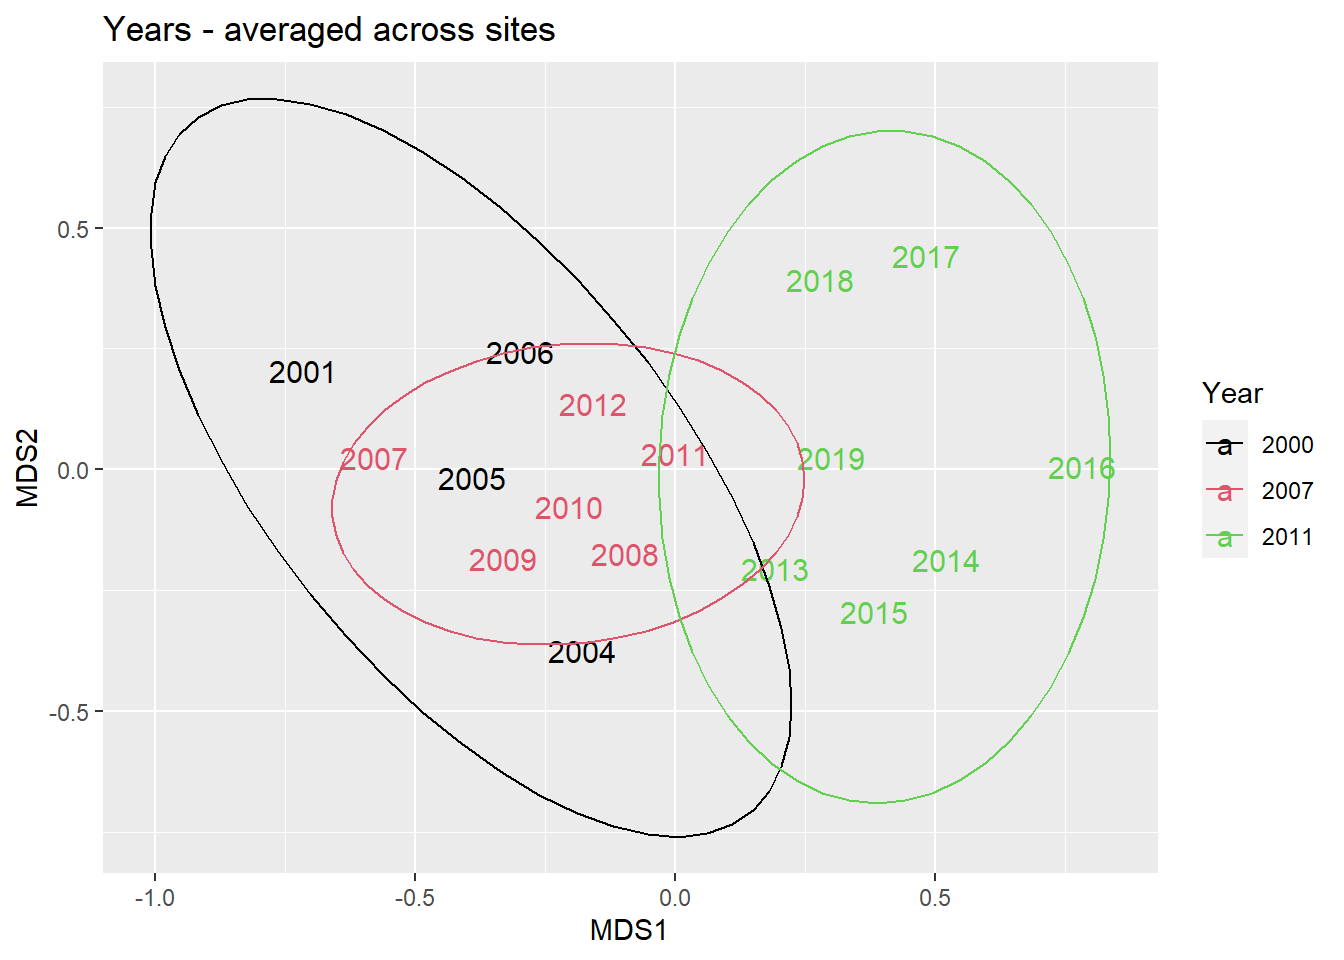
\includegraphics{Workflow_AFRP_files/figure-latex/unnamed-chunk-8-1.pdf}

\begin{Shaded}
\begin{Highlighting}[]
\NormalTok{a =}\StringTok{ }\NormalTok{CPUE_long }\OperatorTok
\StringTok{  }\KeywordTok{filter}\NormalTok{(SPECIES }\OperatorTok{==}\StringTok{ "SMB"}\NormalTok{) }\OperatorTok
\StringTok{  }\KeywordTok{ggplot}\NormalTok{(}\KeywordTok{aes}\NormalTok{(}\DataTypeTok{x =}\NormalTok{ YEAR, }\DataTypeTok{y =}\NormalTok{ (CPUE_seconds))) }\OperatorTok{+}
\StringTok{  }\KeywordTok{geom_point}\NormalTok{() }\OperatorTok{+}
\StringTok{  }\KeywordTok{geom_smooth}\NormalTok{(}\DataTypeTok{method =} \StringTok{"lm"}\NormalTok{) }\OperatorTok{+}\StringTok{ }
\StringTok{  }\KeywordTok{theme}\NormalTok{(}\DataTypeTok{axis.text.x =} \KeywordTok{element_text}\NormalTok{(}\DataTypeTok{angle =} \DecValTok{90}\NormalTok{, }\DataTypeTok{vjust =} \FloatTok{0.5}\NormalTok{, }\DataTypeTok{hjust=}\DecValTok{1}\NormalTok{)) }\OperatorTok{+}\StringTok{   }\KeywordTok{facet_wrap}\NormalTok{(}\OperatorTok{~}\NormalTok{SPECIES)}
\NormalTok{b =}\StringTok{ }\NormalTok{CPUE_long_shore }\OperatorTok
\StringTok{  }\KeywordTok{filter}\NormalTok{(SPECIES }\OperatorTok{==}\StringTok{ "SMB"}\NormalTok{) }\OperatorTok
\StringTok{  }\KeywordTok{ggplot}\NormalTok{(}\KeywordTok{aes}\NormalTok{(}\DataTypeTok{x =}\NormalTok{ YEAR, }\DataTypeTok{y =}\NormalTok{ (CPUE_shoreline))) }\OperatorTok{+}
\StringTok{  }\KeywordTok{geom_point}\NormalTok{() }\OperatorTok{+}
\StringTok{  }\KeywordTok{geom_smooth}\NormalTok{(}\DataTypeTok{method =} \StringTok{"lm"}\NormalTok{) }\OperatorTok{+}\StringTok{ }
\StringTok{  }\KeywordTok{theme}\NormalTok{(}\DataTypeTok{axis.text.x =} \KeywordTok{element_text}\NormalTok{(}\DataTypeTok{angle =} \DecValTok{90}\NormalTok{, }\DataTypeTok{vjust =} \FloatTok{0.5}\NormalTok{, }\DataTypeTok{hjust=}\DecValTok{1}\NormalTok{)) }\OperatorTok{+}\StringTok{   }\KeywordTok{facet_wrap}\NormalTok{(}\OperatorTok{~}\NormalTok{SPECIES)}
\KeywordTok{grid.arrange}\NormalTok{(a,b,}\DataTypeTok{ncol =} \DecValTok{2}\NormalTok{)}
\end{Highlighting}
\end{Shaded}

\includegraphics{Workflow_AFRP_files/figure-latex/unnamed-chunk-9-1.pdf}

\hypertarget{we-can-also-use-the-all_data-to-run-other-fun-analyses}{%
\subsection{\texorpdfstring{We Can also use the \texttt{all\_data} to
run other fun
analyses!}{We Can also use the all\_data to run other fun analyses!}}\label{we-can-also-use-the-all_data-to-run-other-fun-analyses}}

\hypertarget{here-is-average-length-represented-by-habitat-and-overall-trend-through-time}{%
\subparagraph{Here is average length represented by habitat and overall
trend through
time}\label{here-is-average-length-represented-by-habitat-and-overall-trend-through-time}}

While it is not as apparent in these compound graphs, there seem to be
some interesting trends between CPUE and average size through time.

\begin{Shaded}
\begin{Highlighting}[]
\NormalTok{all_data }\OperatorTok
\StringTok{  }\KeywordTok{group_by}\NormalTok{(YEAR, SPECIES, HAB_}\DecValTok{1}\NormalTok{, SEASON) }\OperatorTok
\StringTok{  }\KeywordTok{mutate}\NormalTok{(}\DataTypeTok{avg.length =} \KeywordTok{mean}\NormalTok{(LENGTH, }\DataTypeTok{na.rm=}\NormalTok{T)) }\OperatorTok
\StringTok{  }\KeywordTok{ggplot}\NormalTok{(}\KeywordTok{aes}\NormalTok{(YEAR, }\DataTypeTok{y =}\NormalTok{ avg.length)) }\OperatorTok{+}\StringTok{ }
\StringTok{  }\KeywordTok{geom_point}\NormalTok{(}\KeywordTok{aes}\NormalTok{(}\DataTypeTok{color =}\NormalTok{ HAB_}\DecValTok{1}\NormalTok{)) }\OperatorTok{+}\StringTok{ }
\StringTok{  }\KeywordTok{geom_smooth}\NormalTok{(}\DataTypeTok{method =} \StringTok{"lm"}\NormalTok{) }\OperatorTok{+}\StringTok{ }
\StringTok{  }\KeywordTok{scale_y_continuous}\NormalTok{(}\DataTypeTok{trans=}\StringTok{'log2'}\NormalTok{) }\OperatorTok{+}
\StringTok{  }\KeywordTok{theme}\NormalTok{(}\DataTypeTok{axis.text.x =} \KeywordTok{element_text}\NormalTok{(}\DataTypeTok{angle =} \DecValTok{90}\NormalTok{, }
                                   \DataTypeTok{vjust =} \FloatTok{0.5}\NormalTok{, }\DataTypeTok{hjust=}\DecValTok{1}\NormalTok{)) }\OperatorTok{+}\StringTok{ }
\StringTok{  }\KeywordTok{facet_wrap}\NormalTok{(}\OperatorTok{~}\NormalTok{SPECIES)}
\end{Highlighting}
\end{Shaded}

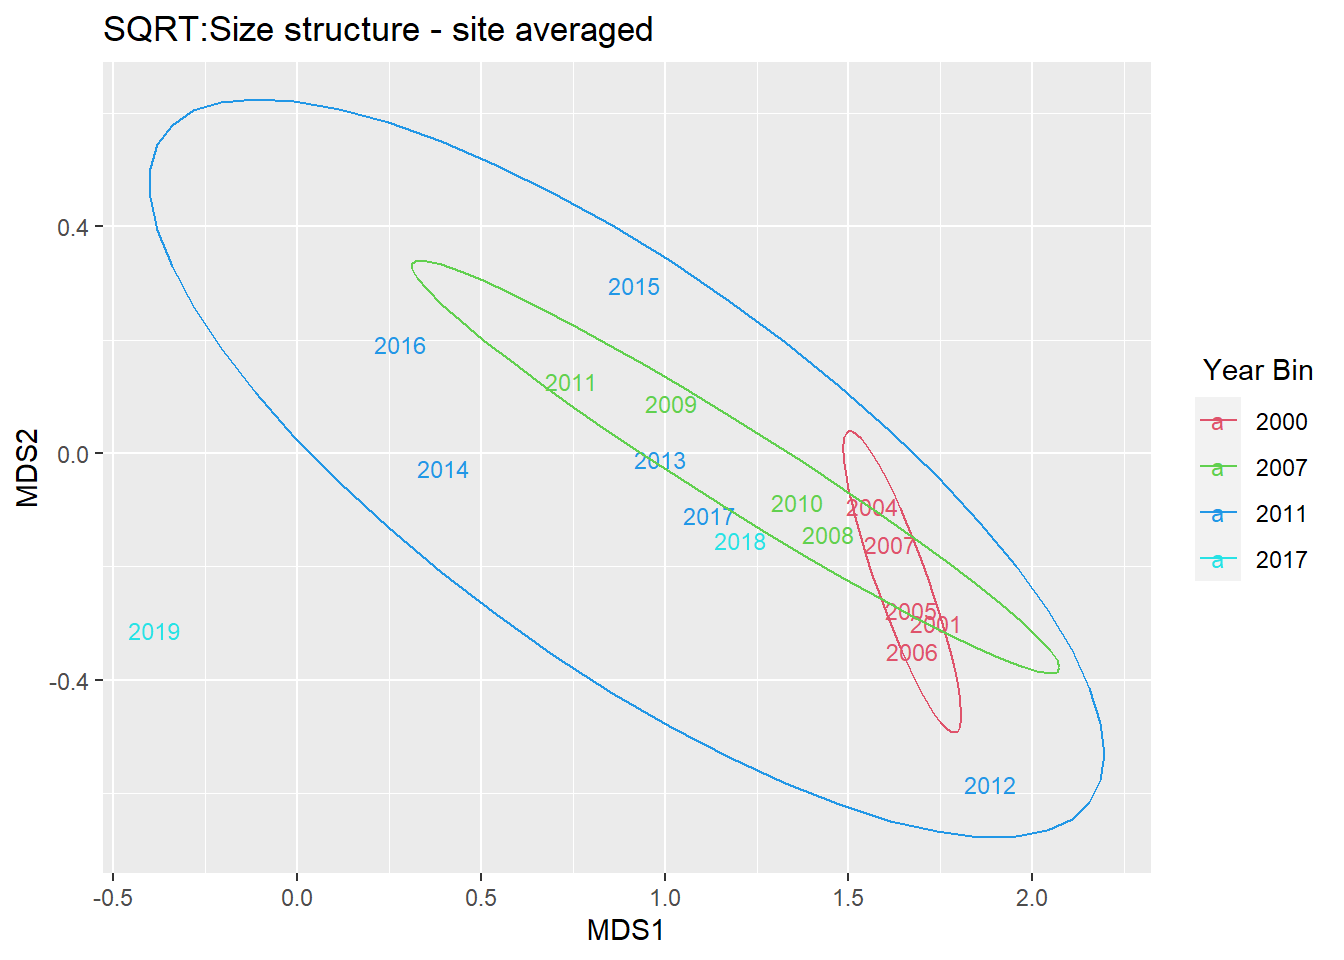
\includegraphics{Workflow_AFRP_files/figure-latex/unnamed-chunk-10-1.pdf}

\hypertarget{checking-to-see-if-the-habitats-are-the-same}{%
\paragraph{Checking to see if the habitats are the
same}\label{checking-to-see-if-the-habitats-are-the-same}}

It looks like all the habitats match up except for Site 1 in HAL that is
just missing that information.

\begin{Shaded}
\begin{Highlighting}[]
\NormalTok{all_data =}\StringTok{ }\KeywordTok{left_join}\NormalTok{(fish, sample, }\DataTypeTok{by =} \StringTok{"YSAMP_N"}\NormalTok{) }\OperatorTok\StringTok{ }
\StringTok{  }\KeywordTok{left_join}\NormalTok{(sites, }\DataTypeTok{by =} \StringTok{"SITE_N"}\NormalTok{) }\OperatorTok\StringTok{ }
\StringTok{  }\KeywordTok{left_join}\NormalTok{(shoreline_length, }\DataTypeTok{by =} \StringTok{"SITE_N"}\NormalTok{) }\OperatorTok
\StringTok{  }\KeywordTok{filter}\NormalTok{(GEAR }\OperatorTok{==}\StringTok{ "BEF"}\NormalTok{) }\OperatorTok
\StringTok{  }\KeywordTok{select}\NormalTok{(WATER, SITE_N, HAB_}\DecValTok{1}\NormalTok{) }\OperatorTok
\StringTok{  }\KeywordTok{unique}\NormalTok{() }\OperatorTok\StringTok{ }
\StringTok{  }\KeywordTok{left_join}\NormalTok{(shoreline_length, }\DataTypeTok{by =} \StringTok{"SITE_N"}\NormalTok{) }\OperatorTok
\StringTok{  }\KeywordTok{filter}\NormalTok{(WATER }\OperatorTok\StringTok{ }\KeywordTok{c}\NormalTok{(}\StringTok{"FBL"}\NormalTok{, }\StringTok{"HAL"}\NormalTok{, }\StringTok{"LML"}\NormalTok{),}
\NormalTok{         SiteNum }\OperatorTok{!=}\StringTok{ "NA"}\NormalTok{) }\OperatorTok
\StringTok{  }\KeywordTok{mutate}\NormalTok{(}\DataTypeTok{check =}\NormalTok{ HAB_}\DecValTok{1} \OperatorTok{==}\StringTok{ }\NormalTok{Habitat) }\OperatorTok
\StringTok{  }\KeywordTok{filter}\NormalTok{(check }\OperatorTok{==}\StringTok{ "FALSE"}\OperatorTok{|}\StringTok{ }\KeywordTok{is.na}\NormalTok{(check))}
\KeywordTok{print}\NormalTok{(all_data)}
\end{Highlighting}
\end{Shaded}

\begin{verbatim}
##   WATER      SITE_N HAB_1 Water SiteNum Shape_Length Habitat check
## 1   HAL BEF.HAL.001  <NA>   HAL       1     51.77533      SW    NA
\end{verbatim}

\hypertarget{hal-brook-trout-data-for-trap-nets}{%
\subsection{HAL Brook Trout Data for Trap
Nets}\label{hal-brook-trout-data-for-trap-nets}}

\begin{Shaded}
\begin{Highlighting}[]
\CommentTok{# Join/Filter ---------}
\NormalTok{all_data =}\StringTok{ }\KeywordTok{left_join}\NormalTok{(fish, sample, }\DataTypeTok{by =} \StringTok{"YSAMP_N"}\NormalTok{) }\OperatorTok\StringTok{ }
\StringTok{  }\KeywordTok{left_join}\NormalTok{(sites, }\DataTypeTok{by =} \StringTok{"SITE_N"}\NormalTok{) }\OperatorTok\StringTok{ }
\StringTok{  }\KeywordTok{separate}\NormalTok{(SITE_N,  }\DataTypeTok{into =} \KeywordTok{c}\NormalTok{(}\StringTok{"GEAR"}\NormalTok{, }\StringTok{"WATER"}\NormalTok{,}\StringTok{"SITE"}\NormalTok{)) }\OperatorTok\StringTok{ }
\StringTok{  }\KeywordTok{filter}\NormalTok{(WATER }\OperatorTok{==}\StringTok{ "HAL"}\NormalTok{,}
\NormalTok{         GEAR }\OperatorTok{==}\StringTok{ "TPN"}\NormalTok{, }
\NormalTok{         YEAR }\OperatorTok{>}\StringTok{ }\DecValTok{1999}\NormalTok{,}
         \CommentTok{### single out or remove specific species}
\NormalTok{         (SPECIES }\OperatorTok{!=}\StringTok{ "NF"} \OperatorTok{&}\StringTok{ }\NormalTok{SPECIES }\OperatorTok{!=}\StringTok{ ""}\NormalTok{), }
\NormalTok{          MONTH }\OperatorTok{>}\StringTok{ }\DecValTok{8}\NormalTok{)}

\CommentTok{## Calculate CPUE information ------}
\NormalTok{CPUE_wide =}\StringTok{ }\NormalTok{all_data }\OperatorTok
\StringTok{  }\KeywordTok{select}\NormalTok{(YSAMP_N, DSAMP_N, YEAR, SEASON, WATER, SITE, SPECIES,}
\NormalTok{         FISH_N, WEIGHT, LENGTH, HAB_}\DecValTok{1}\NormalTok{, GEAR, EFFORT) }\OperatorTok
\StringTok{  }\KeywordTok{group_by}\NormalTok{(WATER, DSAMP_N, YEAR, SITE, SPECIES, EFFORT, HAB_}\DecValTok{1}\NormalTok{) }\OperatorTok
\StringTok{  }\KeywordTok{count}\NormalTok{() }\OperatorTok\StringTok{ }\CommentTok{## Abundance per year, site, species}
\StringTok{  }\KeywordTok{mutate}\NormalTok{(}\DataTypeTok{CPUE_nights =}\NormalTok{ n }\OperatorTok{/}\StringTok{ }\NormalTok{EFFORT) }\OperatorTok
\StringTok{  }\KeywordTok{select}\NormalTok{(}\OperatorTok{-}\NormalTok{n) }\OperatorTok
\StringTok{  }\KeywordTok{pivot_wider}\NormalTok{(}\DataTypeTok{names_from =}\NormalTok{ SPECIES, }\DataTypeTok{values_from =}\NormalTok{ CPUE_nights) }\OperatorTok
\StringTok{  }\KeywordTok{mutate}\NormalTok{(}\KeywordTok{across}\NormalTok{(}\KeywordTok{everything}\NormalTok{(), }\OperatorTok{~}\KeywordTok{replace_na}\NormalTok{(.x,}\DecValTok{0}\NormalTok{)))}

\NormalTok{CPUE_long =}\StringTok{ }\NormalTok{CPUE_wide }\OperatorTok
\StringTok{  }\KeywordTok{pivot_longer}\NormalTok{(}\DataTypeTok{cols =}\NormalTok{ ST}\OperatorTok{:}\NormalTok{RS,}\DataTypeTok{names_to =} \StringTok{"SPECIES"}\NormalTok{, }\DataTypeTok{values_to =} \StringTok{"CPUE_nights"}\NormalTok{ )}

\CommentTok{# ST by site}
\NormalTok{CPUE_long }\OperatorTok
\StringTok{  }\KeywordTok{ggplot}\NormalTok{(}\KeywordTok{aes}\NormalTok{(}\DataTypeTok{x =}\NormalTok{ YEAR, }\DataTypeTok{y =}\NormalTok{ (CPUE_nights))) }\OperatorTok{+}
\StringTok{  }\KeywordTok{geom_point}\NormalTok{() }\OperatorTok{+}
\StringTok{  }\KeywordTok{geom_smooth}\NormalTok{(}\DataTypeTok{method =} \StringTok{"lm"}\NormalTok{) }\OperatorTok{+}\StringTok{ }
\StringTok{  }\KeywordTok{theme}\NormalTok{(}\DataTypeTok{axis.text.x =} \KeywordTok{element_text}\NormalTok{(}\DataTypeTok{angle =} \DecValTok{90}\NormalTok{, }\DataTypeTok{vjust =} \FloatTok{0.5}\NormalTok{, }\DataTypeTok{hjust=}\DecValTok{1}\NormalTok{)) }\OperatorTok{+}\StringTok{  }
\StringTok{  }\KeywordTok{facet_wrap}\NormalTok{(}\OperatorTok{~}\NormalTok{SPECIES)}
\end{Highlighting}
\end{Shaded}

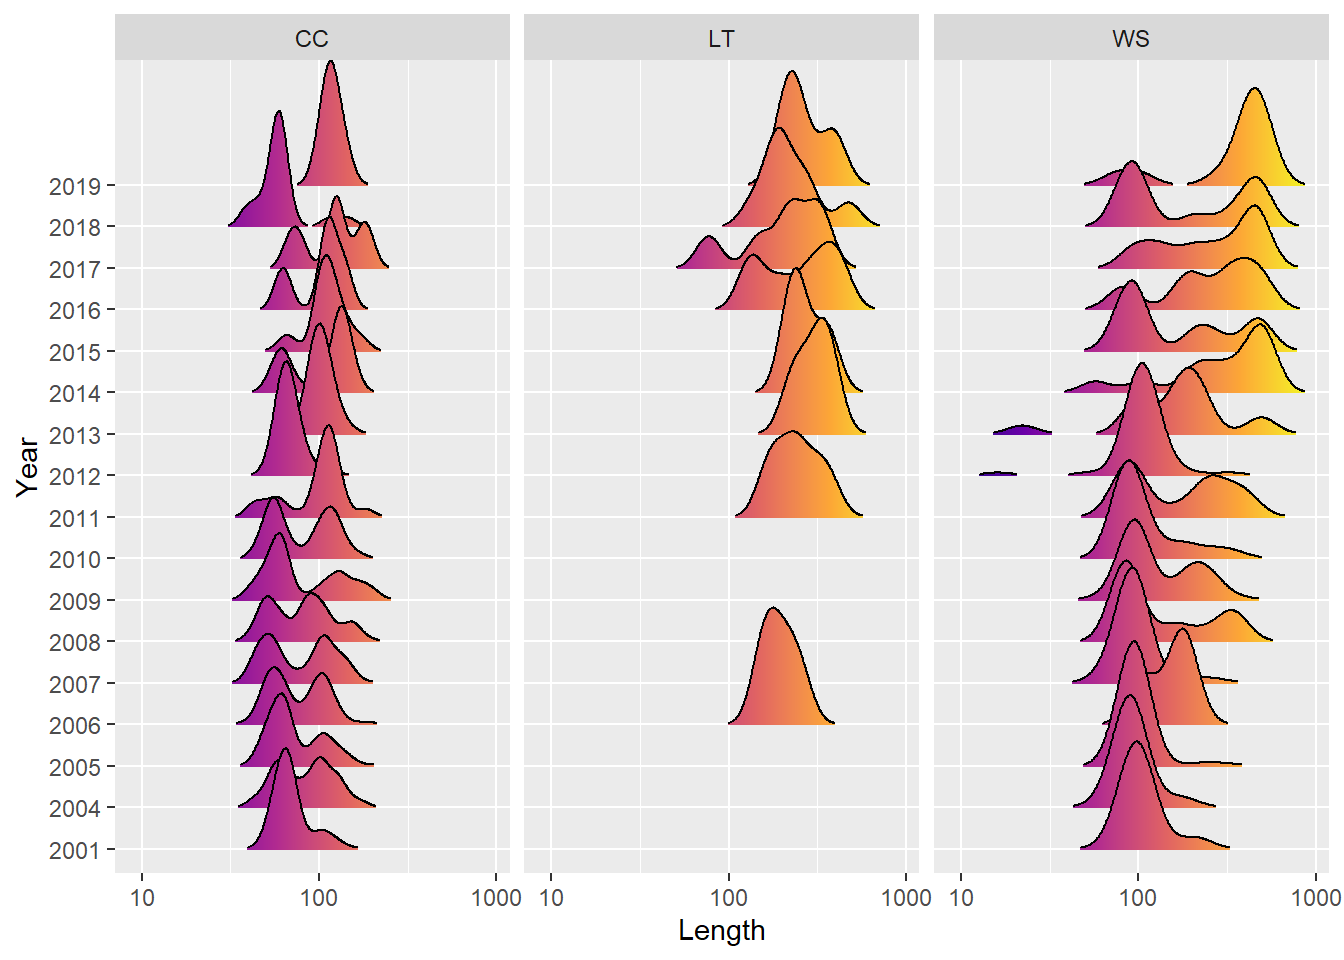
\includegraphics{Workflow_AFRP_files/figure-latex/unnamed-chunk-12-1.pdf}

\end{document}
